%\textcolor{red}{From confirmation report}
%We now consider settings in which the extremal dependence structure is non-stationary, and may change over time.
%For example, meteorological variables observed across spatial locations may exhibit changes in extremal dependence due to shifts in climate regimes, while biomarker measurements collected longitudinally for individuals may display structural changes associated with disease progression, treatment effects, or lifestyle changes \citep{katz2010statistics, Gilles2018, panagoulias2025extreme, Talento2025}.
%In such settings, it is of interest to detect change points or structural breaks in the extremal dependence structure.

%In the existing framework, the multivariate ``groups'' could, in principle, represent different time periods.
%However, this method was not developed to accommodate temporally evolving dependence structures within an already multivariate setting (e.g., spatial), and we assumed that the data within each group was stationary.
%This is limiting in applications where tail dependence is expected to vary over time.
%In environmental contexts, for example, climate change may strengthen or weaken extremal dependence across an entire spatial domain, as suggested by \citet{Zhong2022}, who found that recent Southern European heatwaves have been more widespread than in the past.
%More generally, several types of structural change may occur. 
%In some situations the extremal dependence structure may shift globally across all sites, corresponding to a regime change affecting the entire system. 
%In other settings, only a subset of sites may change their extremal dependence behaviour, for example by switching between clusters of locations with similar tail dependence characteristics.
%Discarding the stationarity assumption and allowing for such temporal changes in extremal dependence is therefore a natural and important extension of our current work.
%It would enable us to identify time periods with distinct spatial patterns of tail dependence, as well as the specific change points at which these transitions occur.
%Therefore, a key focus of this work will be the development of methods for change point detection in multivariate extremal dependence structures, building on the divergence-based framework introduced in our first paper. 

%There has been some previous work on change point detection in multivariate dependence structures, whether in the context of extremes or more generally.
%For example, \citet{McGonigle2025} developed a non-parametric sliding window approach for detecting change points in pairwise extremal dependence. 
%Also, \citet{Alouni2026} developed a Bayesian clustering algorithm for multivariate extremes which utilises a mixture of Dirichlet distributions, and they show how it can be used to temporally cluster negative returns for several S\&P 500 stock sectors, thereby identifying periods of time with similar extremal dependence structures across the sectors.
%In \citet{Agarwal2025}, a likelihood-based method for detecting temporal change points in spatio-temporal data is developed, and applied to daily wind speed data in Ireland, similar to the data we used in our first paper. 
%We hope to build on these existing approaches and also the divergence-based clustering framework developed in our paper to develop a method for detecting change points in multivariate extremal dependence structures, which can be applied to a wide range of datasets and applications.



## Section 2


% Refitting the CE models within each permutation incorporates variation arising from estimation of the extremal dependence structure into the reference distribution.

% We construct a statistical test for detecting a difference in tail behaviour in one or more of the random vectors $\boldsymbol{Y}_1^{(t)},\ldots,\boldsymbol{Y}_D^{(t)}$ based on the conditional extremes models fitted using the data for time blocks $\mathcal{T}_1(\tau)$ and $\mathcal{T}_2(\tau)$. Specifically, the null hypothesis states that the matrix $M^{(t)}$ in \eqref{eq:distance_matrix} remains unchanged throughout the period $\mathcal{T}_1(\tau)\cup\mathcal{T}_2(\tau)$:


%Let $M(T)$ denote the estimated extremal dependence structure for a time block $T$, which could represent a given period of time for which we have sufficient data to fit the CE model and estimate the corresponding divergence matrix.
%A simple way to compare two time blocks $T_1$ and $T_2$ is via the statistic
%\begin{equation} \label{eq:frob}
%D_{\mathrm{obs}} \coloneq \| M(T_1) - M(T_2) \|_{\mathrm{F}},
%\end{equation}
%i.e.\ the Frobenius norm of their difference, defined as
%\[
%  \| A \|_{\mathrm{F}} \coloneq \sqrt{\sum_{i,j} A_{ij}^2}.
%\]
%This statistic captures the overall or global magnitude of change in extremal dependence across all pairs of sites.
%Another option is the infinity, or maximum-entry, norm, defined as
%\[
%  \| A \|_{\infty} \coloneq \max_{i,j}|A_{ij}|,
%\]
% which may better highlight the maximum difference between each matrix, placing greater emphasis on more localised changes in tail dependence.
%which captures the largest difference between corresponding entries of the two matrices and therefore places greater emphasis on localised changes in extremal dependence.
%Critical values for this statistic could be generated via simulation from fitted models to assess whether observed changes represent significant shifts in tail dependence.

%One key question is how large the observed statistic must be to indicate a significant change in extremal dependence.
%A natural way to assess whether the difference between two time periods reflects a genuine structural change, rather than sampling variability in the fitted CE models, is via a permutation test. 
%A permutation test is a non-parametric method for testing hypotheses by comparing the observed test statistic to a reference distribution generated by randomly permuting the data \citep{Good2004}.
%Such procedures are exact when the observations are exchangeable under the null hypothesis.
% One advantage of this approach is that it avoids strong parametric assumptions about the sampling distribution of the divergence matrix, which is unknown, and directly respects the dependence structure of the observed data.
%One advantage of this approach is that it avoids strong parametric assumptions about the sampling distribution of the divergence matrix, which is unknown, and avoids specifying a parametric sampling distribution for the divergence matrix and can accommodate dependence-preserving permutation schemes.

%\subsubsection{Permutation test for temporal changes in extremal dependence}

% \textcolor{red}{Include brief intro to subsubsection introducing screening step and permutation test?}
%Suppose we wish to test for a change in extremal dependence at a candidate split point $\tau$ by comparing two local time blocks immediately before and after the split. 
%Let $T_1$ and $T_2$ denote the corresponding pre- and post-change windows, each of size $n$. 
%We fit the CE model separately in each block, yielding divergence matrices $M(T_1)$ and $M(T_2)$ as defined in Equation~\eqref{eq:distance_matrix} (or their aggregate form in Equation~\eqref{eq:aggregate_matrix}). 

%Our null hypothesis is 
%\[
%H_0:\ \text{the extremal dependence structure is identical in } T_1 \text{ and } T_2.
%\]
%Under this null hypothesis of stationarity, exceedances from the two blocks arise from the same distribution. 
%We therefore generate a reference distribution for $D_{\mathrm{obs}}$ by repeatedly permuting the time indices:
%\begin{enumerate}[label=\arabic*.]
%  \item \textbf{Pool observations:} For a chosen block size $n \le \min\{|T_1|, |T_2|\}$, combine the final $n$ observations from time block $T_1$ and the first $n$ observations from $T_2$ into a single dataset. 
  % \item \textbf{Permute time labels:} Randomly permute the time indices of the pooled observations and reassign them to two pseudo-blocks of size $n$. 
%  \item \textbf{Permute temporal labels:} Randomly reassign the pooled observations, or appropriate dependence-preserving temporal groups, to two pseudo-blocks of size $n$.
%  \item \textbf{Refit CE models:} For the permuted dataset, reapply the exceedance threshold $u$ for each conditioning variable and refit the CE model in each pseudo-block, yielding divergence matrices  $M^{(b)}(T_1)$ and $M^{(b)}(T_2)$, for $b = 1,\dots,B$ permutations.
%\item \textbf{Recompute statistic:} Compute the test statistic
%  \begin{equation} \label{eq:perm_stat}
%    D^{(b)} \coloneq
%    \bigl\| M^{(b)}(T_1) - M^{(b)}(T_2) \bigr\|_{\mathrm{r}},
%    \qquad b = 1,\dots,B, 
%  \end{equation}
%\end{enumerate}
%for the $\mathrm{r}$-norm of choice (Frobenius or infinity).
%As the CE model fitting and divergence calculation are repeated within each permutation, this procedure naturally propagates the estimation uncertainty in the fitted dependence parameters, somewhat analogous to a bootstrapping approach. \textcolor{red}{Remove reference to bootstrap?}
% Refitting the CE models within each permutation incorporates variation arising from estimation of the extremal dependence structure into the reference distribution.

%The empirical $p$-value is then
%\begin{equation} \label{eq:perm_pval}
% \hat{p} =
% \frac{1}{B}
% \sum_{b=1}^B
% \mathbf{1}\!\left\{ D^{(b)} \ge D_{\mathrm{obs}} \right\}.
%\hat{p}
%=
%\frac{
%  1+
%  \sum_{b=1}^{B}
%  \mathbf{1}
%  \left\{
%  D^{(b)}
%  \geq
%  D_{\mathrm{obs}}
%  \right\}
%}{
%  B+1
%}.
%\end{equation}
%A small value of $\hat{p}$ provides evidence that the tail-dependence structure differs between the two time periods. 
%In performing the permutation test, a suitable block size $n$ must be chosen to ensure reliable estimation of the CE model parameters within each time block, while also providing sufficient power to detect changes in extremal dependence.
%Using the same $n$ across all permutations ensures that the sampling variability in the fitted parameters is appropriately reflected in the reference distribution of the test statistic.

%\subsubsection{Sliding-window permutation approach for change point localisation}

% The permutation test above assesses whether a \emph{given} time split corresponds to a change in extremal dependence. 
% % We now extend this idea to estimate the location of an unknown change point.
% We now extend this idea across a sequence of candidate split points to identify periods at which the extremal dependence structure changes.
% 
% Given $N$ total observations and a block size $n < N$, for each candidate change point $\tau \in \{n,\dots,N-n\}$, define the corresponding time blocks
% \[
% T_1(\tau) = \{\tau-n+1,\dots,\tau\}, 
% \qquad 
% T_2(\tau) = \{\tau+1,\dots,\tau+n\},
% \]
% For each $\tau$, we perform the permutation test described above to compute a $p$-value $\hat{p}(\tau)$ as in equation~\eqref{eq:perm_pval}, for the null hypothesis of no change in extremal dependence at $\tau$.
% 
% To avoid running computationally intensive permutation tests at every possible ``split'' point $\tau$, we first identify promising candidate change point locations.
% Define 
% \[
% D_r(\tau) =
% \left\|
%   M\{T_1(\tau)\}
%   -
%   M\{T_2(\tau)\}
% \right\|_r,
% \]
% for $r \in \{\mathrm{F},\infty\}$, as the observed discrepancy between the estimated extremal dependence structures in the two blocks around $\tau$.
% To ``screen'' for these time points, we evaluate $D_r(\tau)$ over a grid of admissible split points from time points $n$ to $N-n$.
% The coarseness of this grid can be adjusted to balance computational cost with the resolution of candidate change point detection.
% Local maxima of the function $D(\tau)$ indicate times at which the extremal dependence structure differs most strongly between the two sides of the split. 
% Let $\{\hat{\tau}_1,\dots,\hat{\tau}_K\}$ denote the $K$ largest local maxima, which we treat as candidate change point regions.
% The function $D(\tau)$ therefore acts as a screening statistic highlighting candidate change point locations.
% 
% Now that we have identified candidate change point locations $\{\hat{\tau}_1,\dots,\hat{\tau}_K\}$, we refine our inference by applying the permutation test described above within a local window around each candidate point.
% \[
% \mathcal{W}_k = \{\tau: \hat{\tau}_k - w \le \tau \le \hat{\tau}_k + w\},
% \]
% for some window half-width $w > 0$. 
% For each $\tau \in \mathcal{W}_k$, we:
% \begin{enumerate}[label=\arabic*.]
%   \item Define blocks $T_1(\tau) = \{\tau-n+1,\dots,\tau\}$ and $T_2(\tau) = \{\tau+1,\dots,\tau+n\}$, as above.
%   \item Compute the observed statistic $D_{\mathrm{obs}}(\tau) = \| M(T_1(\tau)) - M(T_2(\tau)) \|_{\mathrm{F}}$.
% \item Generate its permutation distribution under $H_0(\tau)$ (no change at $\tau$).
% \item Obtain a $p$-value $\hat{p}(\tau)$ as in equation~\eqref{eq:perm_pval}.
% \end{enumerate}
% 
% This produces a local significance profile within each window $\mathcal{W}_k$, mapping $\tau$ to $\hat{p}(\tau)$.
% 
% Within each window $\mathcal{W}_k$, we define the most likely change point as
% \[
% \tilde{\tau}_k = \argmin_{\tau \in \mathcal{W}_k} \hat{p}(\tau),
% \]
% i.e.\ the split point showing the strongest evidence against temporal homogeneity of extremal dependence. 
% % Equivalently, $\tilde{\tau}_k$ corresponds to the most statistically significant peak in $D(\tau)$ after accounting for sampling variability.
% This identifies the split point with the strongest permutation-based evidence against temporal homogeneity, after accounting for sampling variability.
% Furthermore, if $\hat{p}(\tilde{\tau}_k) < \alpha$ for some significance level $\alpha$, we reject the null hypothesis of no change at $\tilde{\tau}_k$, and conclude that there is evidence of a change point in extremal dependence at this time point.
% This two-stage procedure separates effect size from statistical significance: the screening step identifies times at which the estimated extremal dependence structure changes most strongly, while the permutation step determines whether these changes are larger than would be expected under temporal homogeneity.
% 
% \textcolor{red}{Move some of this to discussion}
% The proposed framework provides a flexible starting point for detecting temporal changes in multivariate extremal dependence structures. 
% Several methodological questions remain open. 
% In particular, further work is required to investigate the statistical power of the proposed discrepancy measures under different types of dependence change, to assess the impact of temporal dependence on the validity of permutation procedures, and to develop computationally efficient implementations suitable for large spatial networks. 
% The power of this procedure will depend on both the magnitude of the change in extremal dependence and the number of observations available in each time block.
% Furthermore, in the presence of temporal dependence, block permutations or other dependence-preserving resampling schemes may be required to ensure valid inference.
% Nevertheless, the approach outlined here offers a natural extension of the divergence-based clustering framework developed in the previous chapter and has the potential to provide new tools for identifying structural changes in extremal dependence across time.

%The permutation test above assesses whether a \emph{given} time split corresponds to a change in extremal dependence. 
%We now extend this procedure across a sequence of candidate split points to identify periods at which the extremal dependence structure changes.

%Given $N$ ordered temporal units and a block size $n$, consider candidate change points $\tau \in \{n,\ldots,N-n\}$.
%For each candidate $\tau$, define the adjacent temporal blocks
%\begin{equation}\label{eq:sliding_blocks}
%T_1(\tau)
%\coloneq
%\{\tau-n+1,\ldots,\tau\},
%\qquad
%T_2(\tau)
%=
%\{\tau+1,\ldots,\tau+n\}.
%\end{equation}
%The candidate $\tau$ therefore represents a possible change between temporal units $\tau$ and $\tau+1$.

%We first evaluate the observed discrepancy
%\begin{equation}
%\label{eq:screening_stat}
%D(\tau)
%=
%\left\|
%M\{T_1(\tau)\}
%-
%M\{T_2(\tau)\}
%\right\|_{\mathrm{r}}
%\end{equation}
%over the admissible candidate split points, for $r \in \{\mathrm{F},\infty\}$. 
%The resulting profile provides an initial screening of temporal changes in the estimated extremal dependence structure. 
%In particular, local maxima of $D(\tau)$ identify candidate regions where the fitted dependence structures on either side of the split differ most strongly.

%We then apply the permutation test described above at each feasible candidate $\tau$, yielding a corresponding profile of pointwise $p$-values,
%\[
%\left\{
%\hat{p}(\tau):
%\tau \in \{n,\ldots,N-n\}
%\right\}.
%\]
%A small value of $\hat{p}(\tau)$ indicates that the observed difference between the extremal dependence structures in $T_1(\tau)$ and $T_2(\tau)$ is larger than expected under temporal homogeneity.
%Examining the screening statistic and permutation $p$-values together distinguishes pronounced estimated changes from changes that may instead be attributable to sampling variability.

%\textcolor{red}{precipitation or drought data??}
%When the number of admissible split points is modest, as in our application to Spanish temperature and precipitation data in Section~\ref{sec:app}, permutation testing can be performed over the complete candidate range. 
%In settings with longer time series or substantially larger spatial networks, the screening profile may instead be used to restrict permutation testing to neighbourhoods around its most prominent local maxima, thereby reducing computational cost.

%As changes in environmental dependence structures may occur gradually, a candidate $\tau$ should not necessarily be interpreted as the time of an instantaneous physical transition. 
%Rather, it identifies a division between adjacent periods whose estimated extremal dependence structures differ.





% Summer
%\begin{itemize}
%  \item The two summer periods retain a common large-scale structure, although a number of stations change membership after 1990.
 % \item During 1960--1990, cluster 1 is concentrated more strongly across northern and eastern Spain, while cluster 2 contains many southern and western stations. Cluster 3 occupies an intermediate and geographically mixed position.
  %\item After 1990, several cluster-2 stations located away from the southern coast move to cluster 1, producing a somewhat clearer geographical division between northern/eastern and southern/western locations.
  %\item The summer reorganisation is less extensive than that observed for winter and appears to be driven more strongly by a limited number of stations.
  %\item As for winter, the post-1990 dissimilarity matrix (Supplementary Figure~\ref{fig:diss_summer}) is less clearly block-structured and has a lower overall dissimilarity scale than the earlier matrix.
  %\item The elbow curves in Figure~\ref{fig:elbow} indicate that \(k=2\) is also a plausible representation of the summer structure. In the two-cluster solution, the members of the intermediate cluster are absorbed into cluster 2, indicating weaker separation between these groups than between either group and cluster 1.

  %\item The signed difference matrix between the two summer periods (Supplementary Figure~\ref{fig:sign_matrix_diff})
  % \[
  %     \Delta M^{(\mathrm{S})}
  %     =
  %     M^{(\mathrm{S})}_{1960\text{--}1990}
  %     -
  %     M^{(\mathrm{S})}_{1991\text{--}2024},
  % \]
  %is predominantly positive, providing evidence of an overall reduction in pairwise dissimilarity after 1990.
  %\item Summer contains the largest individual absolute matrix changes among the three divided seasons, with maximum differences of approximately \(0.10\). These changes are concentrated in several prominent rows and columns rather than being distributed uniformly.
  %\item Donostia/San Sebastián-Igeldo and Granada Base Aérea display particularly pronounced positive bands, indicating that their fitted dependence structures became more similar to those at many other stations after 1990.
  %\item Granada Base Aérea also moves from cluster 2 to cluster 1. This transition is consistent with a weakening of the earlier distinction between its original cluster and the remaining dependence regimes.
  %\item The concentration of the summer changes in a limited number of rows and columns is consistent with the comparatively strong change point evidence under the infinity norm.
  %\item Collectively, the summer results suggest partial convergence of the fitted dependence structures while retaining a broad north/east versus south/west spatial organisation.
%\end{itemize}

% Autumn
%\begin{itemize}
    %\item The 1960--1986 autumn clustering resembles the spring solution in retaining a recognisable geographical structure, with distinct groups across western, central and eastern parts of the study region.
    %\item The geographical separation becomes weaker during 1987--2024, with several northern, northeastern, southwestern and Mediterranean stations changing membership.
    %\item This reorganisation is also reflected in the dissimilarity matrices (Supplementary Figure~\ref{fig:diss_autumn}), with the later matrix appearing less distinctly block-structured.

    %\item The autumn signed difference matrix is predominantly positive, indicating that many station pairs have smaller fitted dissimilarities after 1986.
    %\item In contrast to summer, the positive autumn differences are distributed relatively widely throughout the matrix, rather than being dominated by only one or two stations.
    %\item Autumn therefore provides evidence of a broad but generally moderate convergence in fitted extremal dependence structure.

    % \item Before 1987, the clusters are clearly differentiated by the upper DPI quantiles and by \(\widehat{\chi}(0.9)\) and \(\widehat{\bar{\chi}}(0.9)\). Some of this separation persists afterwards, although the marginal DPI differences weaken.
    % \item Stations that change cluster tend to have weaker empirical tail dependence before 1987 but stronger tail dependence afterwards. This apparent reversal provides a possible dependence-based explanation for the observed reassignment, although paired differences should be examined before drawing a firm conclusion.
%\end{itemize}


% Overall interpretation
%\begin{itemize}
    %\item The three seasons with candidate temporal changes exhibit appreciable reorganisation of their estimated spatial clusters, but the form of this reorganisation differs between seasons.
    %\item Winter exhibits the broadest redistribution of cluster membership and a mixture of increasing and decreasing pairwise dissimilarities.
    %\item Summer retains its principal large-scale spatial structure, but contains several large station-specific changes that weaken the separation between some clusters.
    %\item Autumn exhibits a more widespread reduction in pairwise dissimilarity, although its change point evidence is weaker and should be regarded as exploratory.

    %\item Across the divided seasons, the later-period dissimilarity matrices generally exhibit weaker block structure and smaller pairwise dissimilarities. This indicates that the fitted conditional extremal dependence structures became less strongly differentiated across Spain.

    % \item This convergence does not by itself imply that extremal temperature--DPI dependence strengthened. Establishing the direction of dependence change requires paired station-level comparisons of \(\widehat{\chi}(0.9)\), \(\widehat{\bar{\chi}}(0.9)\), or fitted conditional extremes parameters.

    % \item The results likewise do not establish that anthropogenic climate change caused the observed reorganisation, nor that desertification increased. Such conclusions would require separate analysis of marginal drought severity, temporal trends, physical mechanisms and potential confounding factors.

    %\item \textcolor{red}{Below two lines should possibly should go in discussion}
    %\item These results suggest that the regional differentiation of compound temperature--DPI extremes appears to have weakened in the later periods, with locations displaying more similar fitted dependence structures despite retaining some broad geographical organisation.
    %\item One must also be cautious that the periods used to estimate each clustering solution differ, particularly in the case of Winter 1999-2024, providing fewer observations for fitting the conditional extremes models. The increase in uncertainty inherent in using these shorter periods may effect our clustering. 
%\end{itemize}






% % Marginal transformation
% \begin{itemize}
%   \item For both variables, but particularly temperature, there exists some marginal temporal dependence which violates 
%   the assumptions of the conditional extremes model of \citet{Heffernan2007}, namely that of marginal stationarity \todo(Is this correct?)
%   \item Furthermore, there appears to be marginal seasonality present across the year.
%   \item To remove this seasonality, and temporal dependence, we take the data for each individual month across all years, and fit a linear trend by year. 
%   \item By removing this linear trend, we reduce the temporal dependence. 
%   \item Afterwards, we group the data by season, and transform to Laplace margins using the empirical rank transform. 
% \end{itemize}
% 
% % CE
% \begin{itemize}
%   \item For our fitted CE models, we observed good empirical performance, in terms of subsequent clustering solutions exhibiting strong spatial contingency, at the 80th dependence quantile. \todo{Need to do sensitivity analysis}
%   \item All subsequent calculations are also done on the aggregated dissimilarity matrix. \todo{Need to look into others as well}
% \end{itemize}
% 
% % Screening/change point setup
% \begin{itemize}
%   \item For our screening step and change point detection algorithm, we must perform our permutation test slightly differently to in our simulation study. 
%   \item \todo{Describe how we permutate by `season year', define season year, etc}
%   \item There is an implicit bias-variance tradeoff in the block length used.
%   \item Empirically, we saw good performance with a block length of 25 years, since for a lesser number of years we saw some very large dissimilarities, while 
%     a greater number of years left us with little perspective change point timepoints/season years to test at. 
% \end{itemize}

% Marginal preprocessing
%\begin{itemize}
%  \item The conditional extremes framework is applied after transforming each variable to a common marginal distribution. 
  %\item Consequently, systematic changes in the marginal distributions over time could otherwise be confounded with changes in the extremal dependence structure.
  %\item Both variables exhibit seasonal variation, while weekly maximum temperature in particular also displays a long-term marginal trend. 
  %\item We therefore preprocess the marginal distributions before fitting the conditional extremes models.
  %\item At each station, and for each variable, we consider observations from each calendar month separately and fit a linear trend in year. 
  %\item The estimated trend is removed from the observations for that month. 
  %\item Treating months separately allows the magnitude of the temporal trend to vary throughout the year while accounting for the pronounced marginal seasonality.
  %\item This detrending removes an estimated linear change in the location of each monthly marginal distribution; it does not imply that all temporal dependence has been removed. 
  %\item In particular, some short-range dependence may remain between successive weekly observations, and consecutive values of the 13-week drought index are constructed from overlapping precipitation windows.
  %\item Following detrending, the observations are grouped by meteorological season. 
  %\item For each station and variable, the resulting seasonal observations are transformed to standard Laplace margins using the empirical rank transform.
  %\item The conditional extremes and change point analyses are then performed separately for winter, spring, summer and autumn.
%\end{itemize}

% Conditional extremes specification
%\begin{itemize}
%\item We fit the conditional extremes model of \citet{Heffernan2004} using a common dependence threshold equal to the theoretical 80th percentile of the standard Laplace distribution. 
%\item The same threshold is used for both variables, at every station, in both temporal blocks and at every candidate change point. 
%\item This ensures that exceedances have a common interpretation throughout the analysis.
%\item The 80th-percentile threshold provided a satisfactory empirical compromise between restricting attention to the joint tail and retaining enough exceedances for stable model estimation. 
%\item In particular, the resulting clustering solutions exhibited clear spatial contiguity. \textcolor{red}{Add a sensitivity analysis for the dependence threshold.}
%\item The Monte Carlo approximation used to construct the pairwise dissimilarities employs the same sample from the standard Laplace distribution in every temporal comparison. Holding this sample fixed avoids introducing additional Monte Carlo variation between candidate change points. \textcolor{orange}{CR: This may be too niche a comment to make here.}
%\item The conditional fits from the two conditioning directions are combined into the aggregated dissimilarity matrix defined in Section~\ref{sec:method}. \textcolor{red}{Test for others}
%\item All screening, testing and clustering calculations reported below use this matrix. \textcolor{red}{Confirm terminology and add sensitivity results for the alternative dissimilarity matrices, if required.}
%\end{itemize}

% Screening and change point-test specification
%\begin{itemize}
  %\item We use the season-year organisation defined in Section~\ref{sec:data} and apply the permutation procedure in Section~\ref{subsec:cp} separately within each season.
  %\item At candidate season-year $t$, the two temporal blocks contain the 25 season-years ending at $t$ and the 25 season-years beginning at $t+1$, respectively.
  %\item In each pointwise permutation, the 50 complete season-years are pooled and randomly reassigned to two pseudo-blocks of 25 season-years each, using the same reassignment for both variables and all 40 stations.
  %\item The validity of this permutation procedure relies on treating season-years as exchangeable under the null hypothesis of no change in the extremal dependence structure. 
  %\item Although permuting complete season-years preserves within-year dependence, it does not preserve any residual dependence between successive season-years.
  %\item Permuting complete season-years preserves the dependence between observations within a season-year and the spatial correspondence between stations.
%\end{itemize}

% Choice of block length
%\begin{itemize}
%\item The choice of block length involves a bias-variance trade-off. 
%\item Shorter blocks provide better temporal localisation but contain fewer threshold exceedances, resulting in unstable or failed conditional extremes fits. 
%\item Longer blocks provide more stable estimates but leave fewer feasible candidate change points and smooth changes over a wider temporal interval.
%\item We investigated block lengths of 15, 20, 25 and 30 season-years. 
%\item With 15-year blocks, many candidate comparisons failed because at least one conditional fit contained too few exceedances. 
%\item Twenty-year blocks were reliable for winter but produced substantial failure rates for several other seasons. 
%\item All candidate comparisons fitted successfully with 25-year blocks. 
%\item Increasing the length to 30 years also produced stable fits, but left only two to five candidate change points per season.
%\item We therefore use 25 season-years on either side of each candidate throughout the primary analysis. 
%\item This was the shortest common block length that produced stable fits across all seasons while retaining a useful range of candidate change points. \textcolor{red}{Present the alternative block lengths as a sensitivity analysis or in the supplementary material(?).}
%\end{itemize}

% \todo{Say something about uses of spectral norm, even just for notes}
% % Point of spectral norm: 
% \begin{itemize}
%   \item Figure~\ref{fig:app_screen} shows the results of the screening step for each season for the Frobenius, Infinity and Spectral norms, respectively. \todo{Need for spectral?}
%   \item Several ``peaks'', defined as $\ldots$, are observed across all seasons and choices of norm. \todo{Define how we determine peaks}
%   \item \todo{Describe screening results each season separately (say where peaks are, comment on scale on y-axis and max values)}       
%   \item While this screening step identifies several years of particular interest, there are a sufficiently small number of candidate change point years to perform our change point algorithm at every timestep.
% \end{itemize}

%\begin{itemize}
%\item We first perform a computationally less intensive screening step, in which the observed discrepancy between the two estimated dissimilarity matrices is calculated at every feasible candidate season-year without generating a permutation distribution.
%\item Figure~\ref{fig:app_screen} presents the screening statistics for each season using the Frobenius, infinity and spectral norms. 
%\item As discussed in Section~\ref{subsec:cp}, these norms provide complementary summaries of the difference between the dissimilarity matrices on either side of a candidate change.
%\item The three norms have different numerical scales, and their absolute values should therefore not be compared directly. 
%\item Instead, we compare the timing and relative prominence of features in their respective screening curves.
%\item Red points in Figure~\ref{fig:app_screen} identify local peaks. 
%\item For a given norm $(T)$, an interior candidate season-year $(t)$ is classified as a local peak when
%\[
%T(t)>T(t-1)
%\qquad\text{and}\qquad
%T(t)\geq T(t+1).
%\]
%The first and final candidate years are not classified as local peaks because they cannot be compared with candidates on both sides.
%\end{itemize}

%\begin{itemize}
%\item For winter, all three norms increase during the late 1990s and exhibit a prominent shared peak in 1998. 
%\item A smaller common peak is present around 1992. 
%\item The agreement among the norms makes the late-1990s period a particularly notable candidate region.
%\item For spring, the clearest screening peak occurs around 1992, for all norms. 
%\item Smaller local peaks occur around 1989 and 1997.
%\item For summer, the screening curves contain several prominent peaks. 
%\item The largest norm values occur in 1988, with further substantial peaks in 1992 and 1997. 
%\item For Autumn, the screening results are less concentrated around a single candidate year. 
%\item The Frobenius curve has local peaks around 1990 and 1996, while the infinity and spectral curves identify broadly similar candidate regions during the late 1980s or early 1990s and the mid-1990s. 
%\item The precise locations of the peaks are less consistent across norms than for winter, spring or summer.
%\item Across the four seasons, the largest Frobenius norm screening value occurs for summer around 1988. \textcolor{red}{Cite exact value}
%\item The clearest agreement among all three norms occurs around 1992 for spring and around 1998 for winter.
% \item The screening curves identify periods in which the estimated extremal dependence structure differs most strongly between the two temporal blocks, but they do not provide measures of statistical significance. 
% \item Moreover, statistics at neighbouring candidate years are strongly dependent because adjacent 25-year windows share almost all of their observations.
%\item Although the screening step highlights several candidate regions of particular interest, the total number of feasible candidate season-years is sufficiently small to apply the permutation test at every candidate. 
%\item We therefore retain the complete candidate range rather than restricting the formal analysis to the local screening peaks.
% \end{itemize}

% \begin{itemize}
%   \item Figure~\ref{fig:app_cp} shows, for each season, the p-values of the change point detection algorithm with 200 permutations at each season year, for each choice of norm. 
%   \item No change points are observed for Spring and Autumn at the 5\% significance level, for any season year or norm choice \todo{May have to revise, change point is found for Autumn! For now act as if not}
%   \item For Winter, the infinity norm finds change points at the season years from 1996 to 1999, while the other norms find change points at 1997 and 1998 only. 
%   \item For Summer, the infinity norm
%   \item It is interesting that the infinity norm is most sensitive to the identified change points. 
%   \item This may suggest that the changes are sometimes more localised than globally found. 
%   \item Furthermore, for Summer post 1994, the infinity norm produces the largest p-values, giving extra surety to the conclusion that local changes do not occur around the season years 1994-1998. \todo{Tidy up this conclusion, if even needed/desired!}
%   \item For many of the season years determined to be change points for Summer and Winter, the other norm choices also produce significant p-values, and so are in agreement with the infinity norm. 
% \end{itemize}
% 
% \begin{figure}[htb]
%     \centering
%     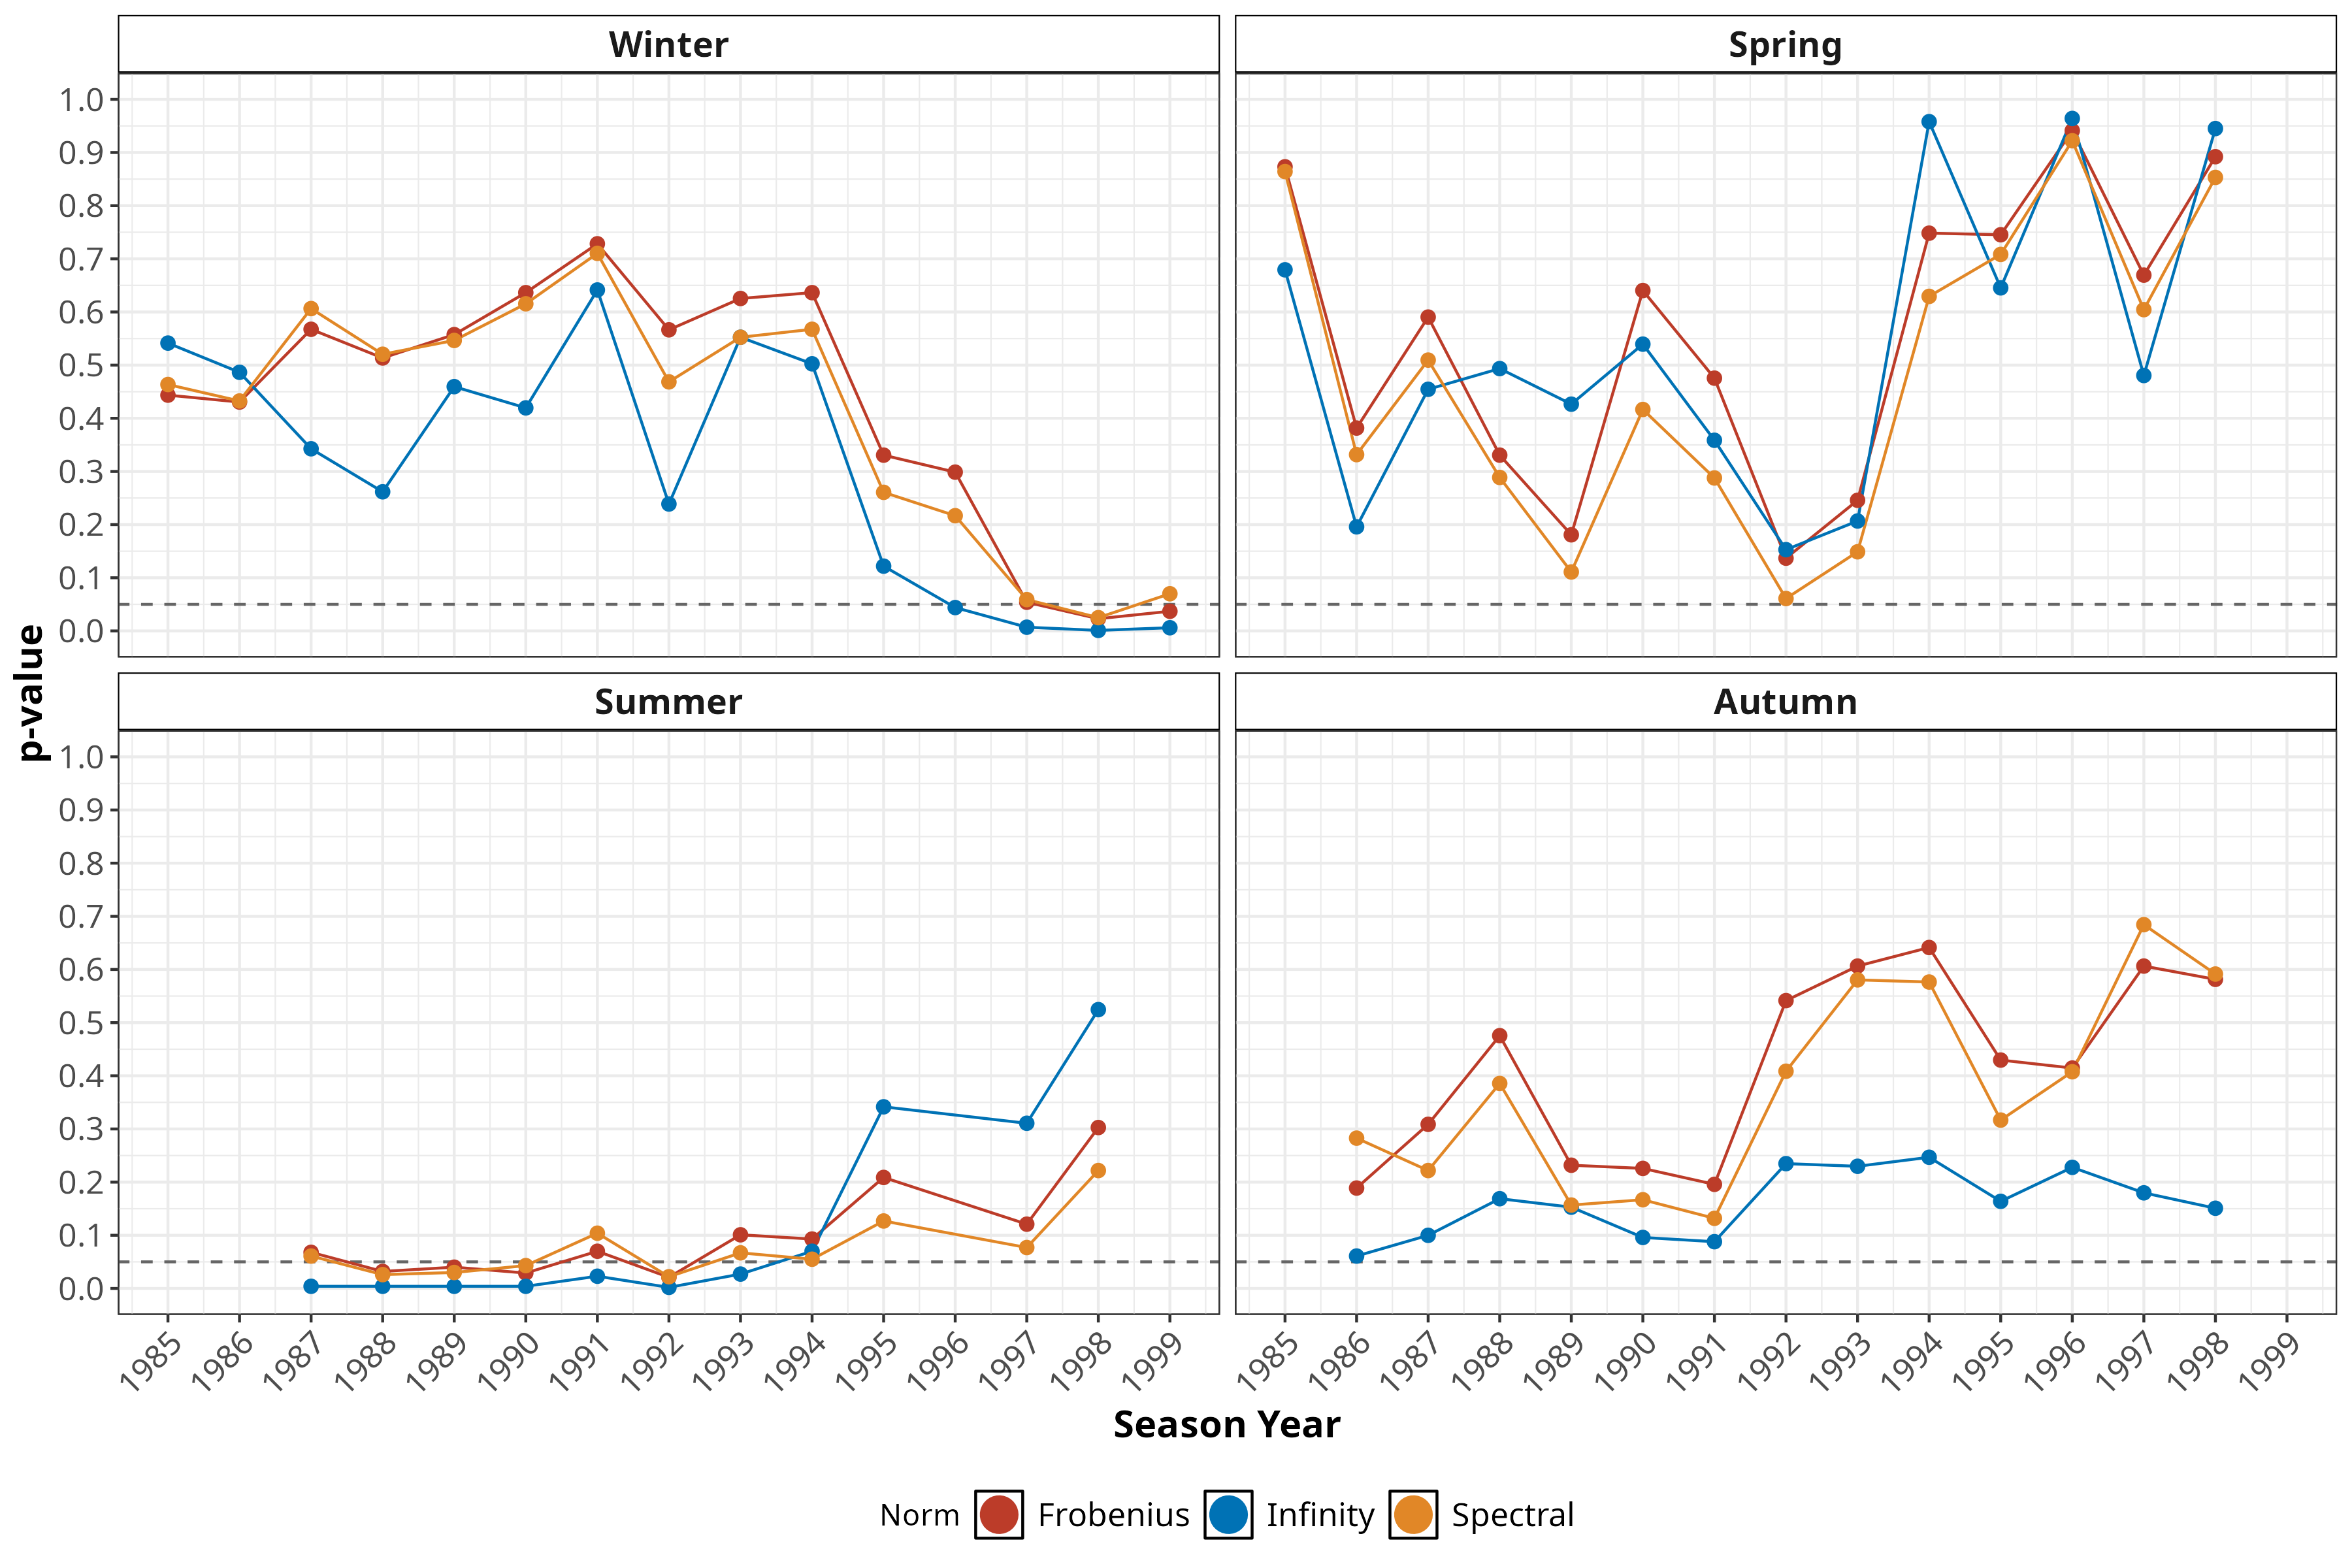
\includegraphics[width = 0.9\linewidth]{plots/change.png}
%     \caption{ 
%       Insert here
%     }
%    \label{fig:app_cp}
% \end{figure}

%\begin{itemize}
%\item We next apply the permutation test at every feasible candidate season-year. 
%\item For each candidate and norm, the null distribution is estimated using 1000 permutations of complete season-years between the two 25-year blocks.
%\item Figure~\ref{fig:app_cp} shows the resulting pointwise Monte Carlo p-values for the Frobenius, infinity and spectral norms. 
%\item A candidate season-year $(t)$ represents a possible change between season-years $(t)$ and $(t+1)$, and the horizontal dashed line denotes the pointwise 5\% significance level.
%\item The p-values in Figure~\ref{fig:app_cp} are pointwise: each tests a change at one specified candidate season-year. 
% \item Because the procedure examines multiple candidate years and three norms, values below 0.05 should initially be interpreted as pointwise evidence rather than as multiplicity-adjusted confirmation of a change point. \todo{Replace or supplement these results with Holm-adjusted p-values or a permutation maximum-statistic test for the final analysis.}
%\end{itemize}

%\begin{itemize}
%\item For spring, none of the three norms produces a pointwise p-value below 0.05. 
%\item The smallest values occur around 1992, in agreement with the dominant feature identified during screening, but remain above the pointwise significance threshold.

% \item For autumn, the infinity norm produces an isolated pointwise-significant result at the beginning of the candidate range, around 1986. \todo{Add change point to re-clustering plot!}
% \item The Frobenius and spectral norms provide no corresponding evidence at this candidate, and no later autumn candidate is significant. 
% \item This isolated result should therefore be interpreted cautiously, particularly because it occurs at the boundary of the candidate range and is not supported by the other norms.
%\item Also for Autumn, none of the three norms produces a pointwise p-value below 0.05, although the infinity norm came very close for 1986, the year with the highest test statistic in our screening step. \textcolor{red}{May have to rewrite slightly, as Autumn now has a 5\% change point (even here, it's significant at the 10\% level)} \textcolor{orange}{CR: I would say we stick with the 5\% level, because it is consistent with our cluster analysis.}
%\item For winter, the infinity norm provides pointwise evidence of a change over the period 1996--1999. 
%\item The spectral norm supports a narrower region around 1997--1998, while the Frobenius norm is significant in 1998. 
%\item Thus, all three norms identify 1998, and the overall pattern provides consistent evidence for a change in the winter extremal dependence structure during the late 1990s.
%\item For summer, the infinity norm produces pointwise-significant p-values over an extended period from approximately 1987 to 1993. 
%\item The Frobenius and spectral norms support narrower subsets of this region, with particularly small p-values around 1988-1990 and 1992.
%\item The agreement among the norms indicates that the early-1990s signal is not confined to a single choice of discrepancy statistic.
%\item After approximately 1994, the summer p-values generally increase, particularly for the infinity norm.
%\item These results provide no pointwise evidence for a change at these later candidates. 
%\item However, the relatively large p-values should not be interpreted as affirmative evidence that the dependence structure is unchanged; they indicate only that the observed discrepancies are not unusual under the corresponding permutation null distributions.
%\end{itemize}

%\begin{itemize}
%\item The infinity norm identifies broader pointwise-significant candidate ranges than the Frobenius and spectral norms for both summer and winter. 
%\item As discussed in Section~\ref{sec:method}, this may indicate that some changes are more pronounced in particular entries of the dissimilarity matrix than across its entire structure.
%\item Nevertheless, the principal summer and winter candidate regions are supported by more than one norm. 
%\item In particular, all three norms provide pointwise evidence around 1990 for summer and around 1998 for winter.
%\item Taken together, the results suggest candidate changes in the summer extremal dependence structure during the late 1980s or early 1990s and in the winter structure during the late 1990s. 
%\item No comparable evidence is found for spring or autumn. % , while the isolated autumn infinity-norm result requires further assessment after accounting for the scan over candidate years.
%\end{itemize}




%\subsection{Clustering Results}\label{subsec:app_clust}

% % Old!
% \begin{itemize}
% \item We finally examine how the detected changes affect the spatial clustering of the fitted extremal dependence structure. 
% \item For each fitted conditional extremes model, the aggregated dissimilarity matrix is used to partition the 40 stations into three clusters using the clustering procedure described in Section~\ref{sec:method}.
% \item As the change point analysis provides no consistent evidence of a change in spring or autumn, we refit the conditional extremes model to the complete time series for these seasons. 
% 
% \item For summer, the pointwise tests identify a broader candidate change region during the late 1980s and early 1990s. 
% \item We use 1990 as a representative division within this region and fit separate models to season-years 1960--1990 and 1991--2024.
% 
% \item For winter, the three norms provide their clearest common evidence at season-year 1998. 
% \item We therefore fit separate models to winter season-years 1960--1998 and 1999--2024.
% 
% \item These divisions treat a candidate (t) as a change between season-years $(t)$ and $(t+1)$. \textcolor{red}{Confirm or update the selected divisions after completing the multiplicity-adjusted change point analysis.}
% \end{itemize}
% 
% \begin{itemize}
% \item Figure~\ref{fig:app_clust} presents the resulting spatial clusterings. 
% \item Although station coordinates and elevation do not directly determine the clustering assignments, the fitted clusters exhibit substantial spatial coherence. 
% \item Neighbouring stations are frequently assigned to the same cluster, suggesting that the estimated extremal dependence structure contains a strong geographical component.
% 
% \item The spring clustering broadly separates groups of stations along the northern and Mediterranean coasts (in blue) from groups in the western (orange) and central interior (red). 
% \item Nevertheless, the boundaries are not determined solely by physical proximity, with some geographically separated stations assigned to the same dependence cluster.
% 
% \item The autumn clustering exhibits a stronger broadly coastal--interior structure. 
% % \item Several stations along the northern and eastern coasts are grouped together, similar to the spring clustering, while clusters containing central, western and southwestern stations form comparatively coherent regional groupings.
% \item Several stations along the northern and eastern coasts are grouped together, similar to the spring clustering, while the other two clusters comprise locations in the west/south-west and elsewhere, respectively. 
% 
% \item For summer, the two fitted periods retain some common large-scale structure.
% \item However, a number of stations change their clustering relationships after 1990, most visibly in northwestern Spain, along the southern coast and across parts of the western interior. 
% \item The summer change point therefore corresponds to a reorganization of particular regional relationships rather than a complete replacement of the earlier clustering structure.
% 
% \item The winter clustering, in contrast, changes more extensively across the 1998 division. 
% \item In particular, the post-1998 fit produces a different grouping of many stations along the northern coast, in the western and central interior, and along the Mediterranean coast. 
% \item This broader spatial reorganisation, as opposed to the more localised changes seen in summer, is consistent with the late-1990s signal being identified by all three norms in the change point analysis.
% \end{itemize}

%\begin{figure}[htb]
%\centering
%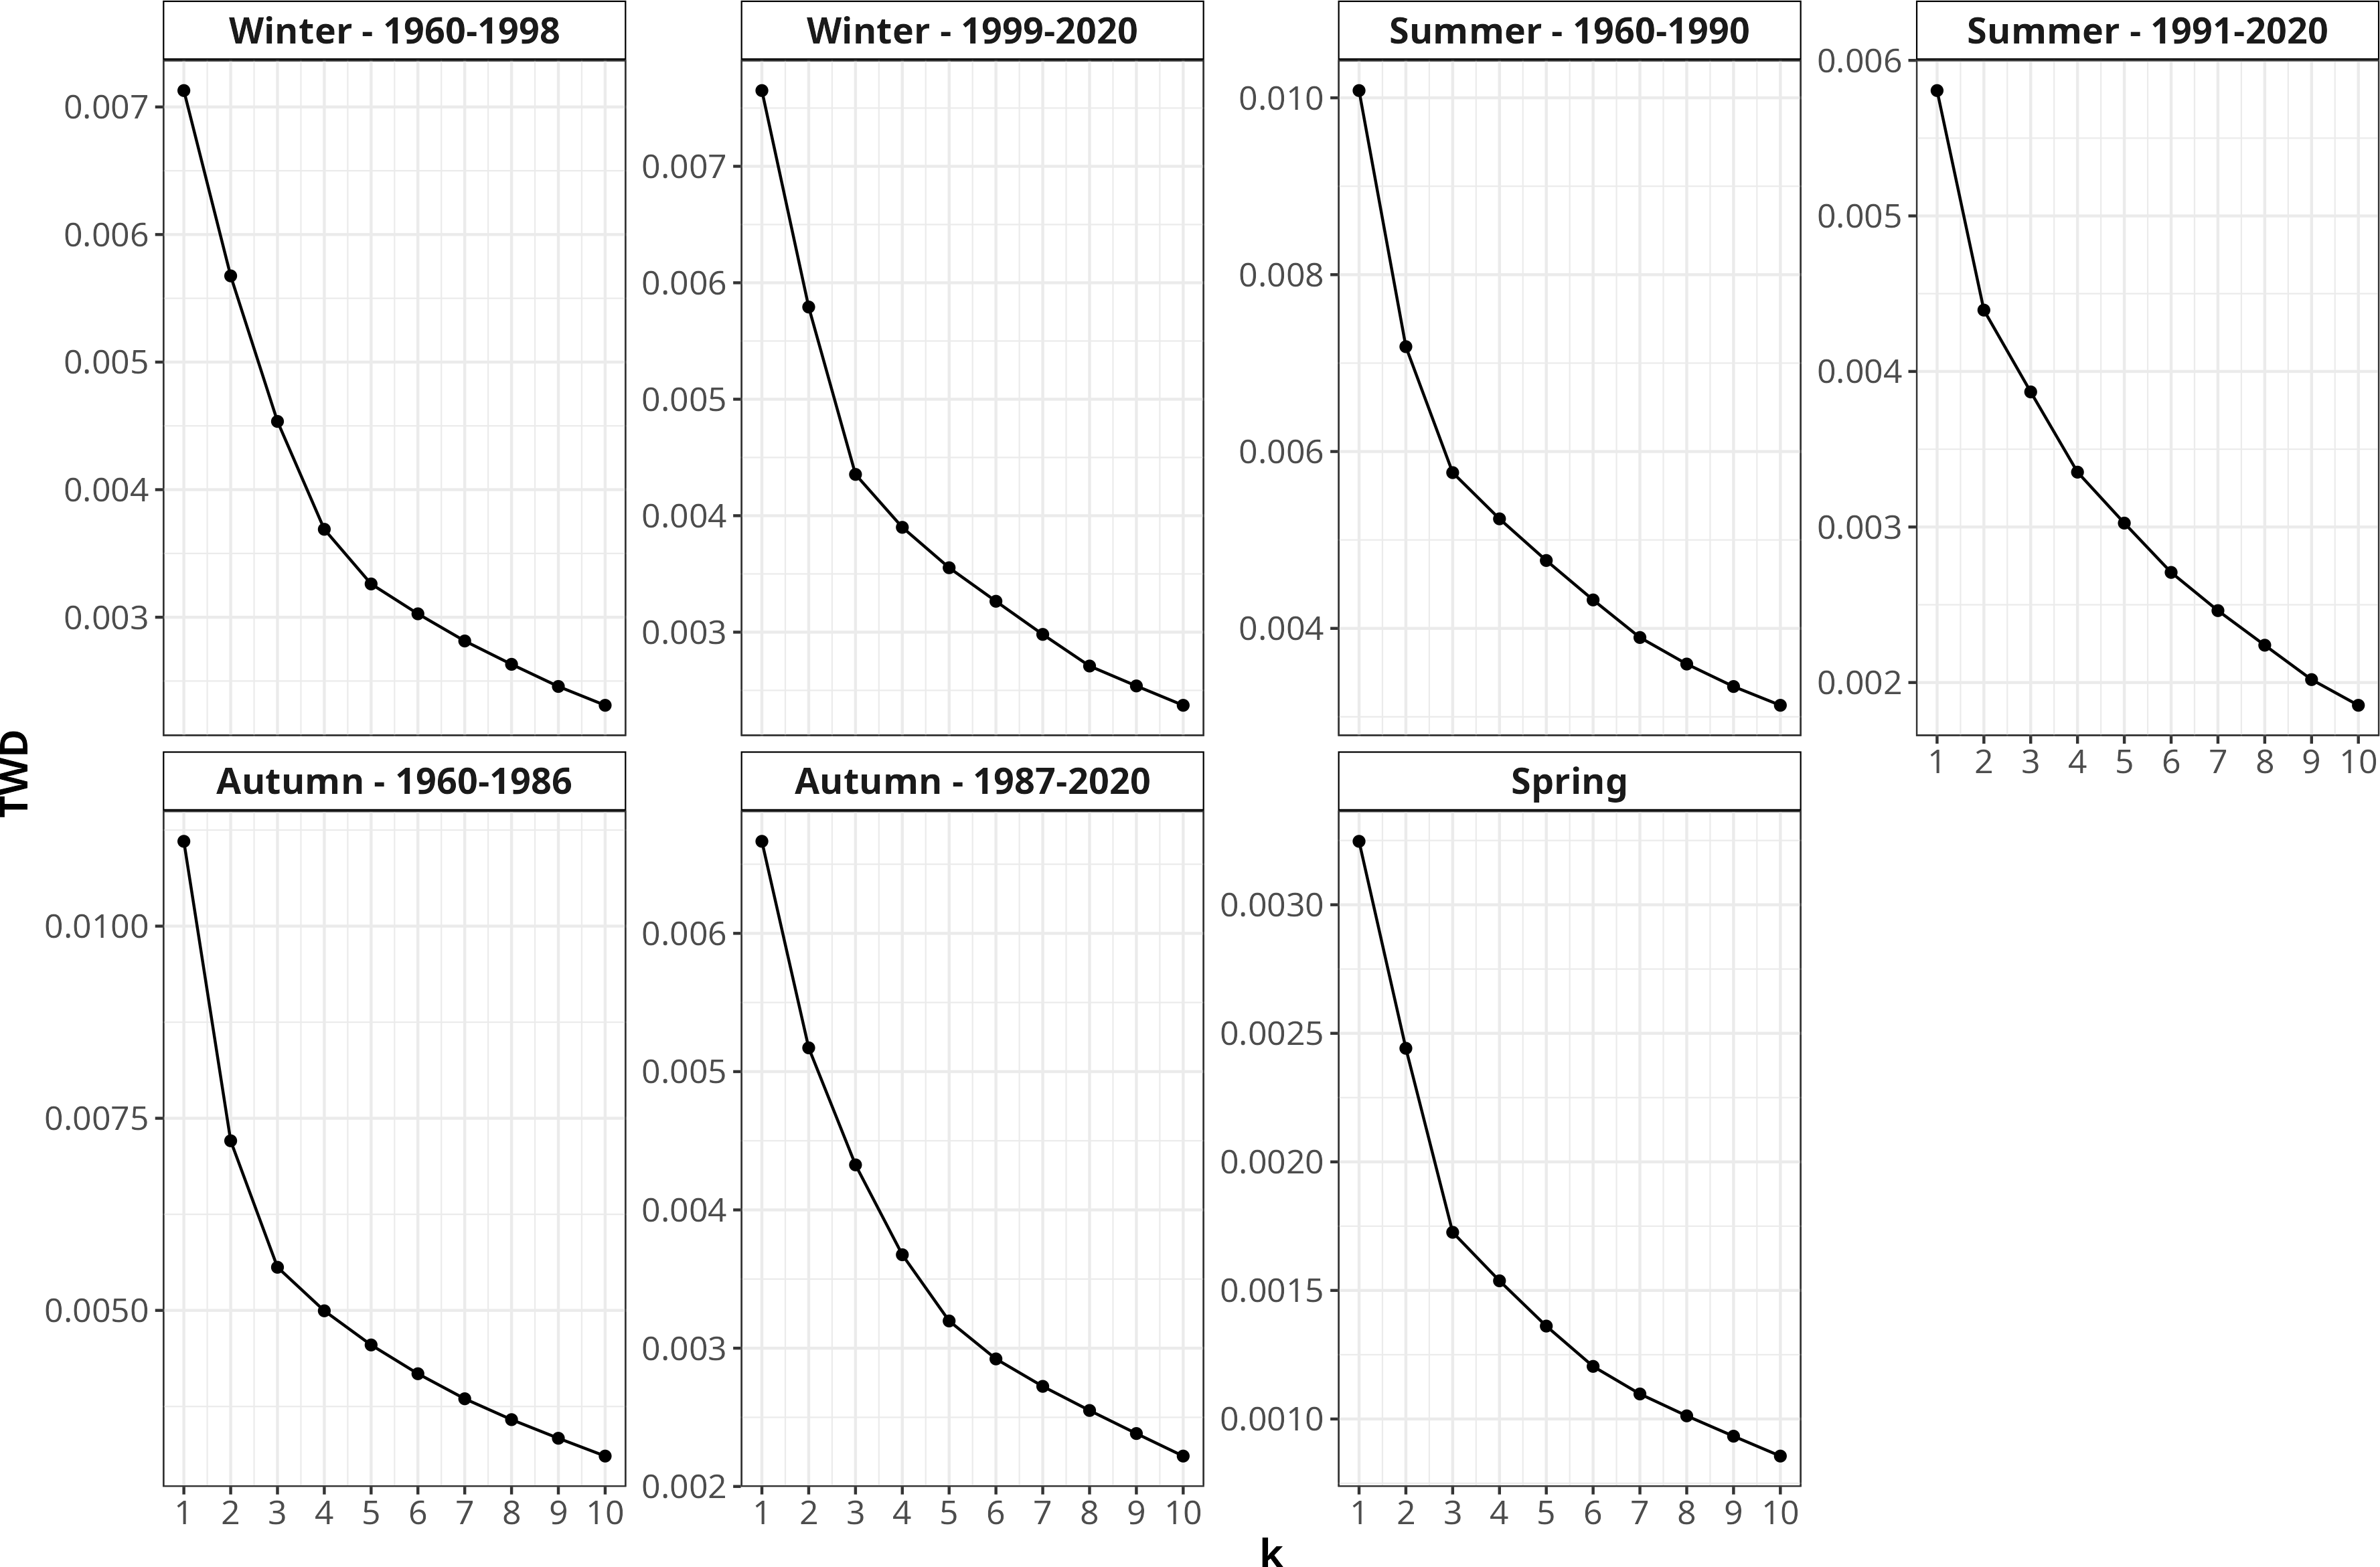
\includegraphics[width=0.9\linewidth]{plots/twgss_dqu_0.8_all_trim.png}
% \caption{
% }
%\caption{
%``Elbow'' plots of the total within-group dissimilarity (TWD) against the number of clusters $k$ for the estimated clusters, obtained using the aggregated dissimilarity matrix for each season and their respective change point divisions.
%\textcolor{red}{Are elbow plots briefly alluded to in methods?}
%}
%\label{fig:elbow}
%\end{figure}

% Setup and elbow plots
%\begin{itemize}
    %\item We finally investigate how the detected temporal changes are reflected in the spatial clustering of the fitted extremal dependence structures.
    %\item For each fitted conditional extremes model, the aggregated dissimilarity matrix is used to partition the 40 stations into three clusters using the procedure described in Section~\ref{sec:method}.
    %\item For summer, the pointwise tests identify a broader region of evidence during the late 1980s and early 1990s. We use 1990 as a representative division and fit separate models to season-years 1960--1990 and 1991--2024.
    %\item For winter, the clearest common evidence across the three matrix norms occurs at season-year 1998. Separate models are therefore fitted to season-years 1960--1998 and 1999--2024.
    %\item For autumn, the infinity norm identifies possible evidence of a change at 1986 at the 10\% pointwise significance level. We consequently examine the periods 1960--1986 and 1987--2024 as an exploratory sensitivity analysis.
    %\item These divisions treat a candidate (t) as a change between season-years $(t)$ and $(t+1)$.
    %\item The change point analysis provides no consistent evidence of temporal change in spring. We therefore fit a single conditional extremes model to the complete spring record.
    %\item The total within-cluster dissimilarity curves for each season and their respective divisions are shown in Figure~\ref{fig:elbow}.
    %\item Together, they generally support $k=3$ as an interpretable compromise between parsimony and within-cluster homogeneity.
    %\item However, as $k=2$ and $k=4$ also appear to be plausible for some elbow plots, we provide the corresponding clustering solutions in the Supplementary Material (Figures~\ref{fig:app_clust_k2}--~\ref{fig:app_clust_k2_4_spring}).
%\end{itemize}



% \subsection{Additional Results}
% 
% \subsubsection{Dissimilarity Matrices}
% 
% \begin{itemize}
% \item Signed differences are calculated as $D_{\mathrm{before}}-D_{\mathrm{after}}$.
% \item Positive differences therefore indicate that a pair of locations became more similar after the change point, whereas negative differences indicate that it became more dissimilar.
% \item Winter contains a mixture of positive and negative differences, suggesting heterogeneous restructuring rather than a uniform change.
% \item The Winter changes are concentrated in particular rows and columns, indicating that a limited number of locations contribute disproportionately to the change.
% \item Summer differences are predominantly positive, suggesting a general reduction in pairwise dissimilarity after 1990.
% \item Summer also contains the largest individual absolute differences, reaching approximately $0.10$.
% \item Autumn differences are also predominantly positive but are more widely distributed throughout the matrix, suggesting a relatively widespread convergence in fitted dependence structure.
% \item Colour intensity should not be compared directly between seasons because the panels use different colour-scale limits.
% \end{itemize}